\chapter{Implementation details}
\label{chapter4}
\thispagestyle{empty}

\section{System architecture}
\paragraph{}
Our tool is entirely based on PIN, a binary instrumentation framework developed by Intel. It lets us to have the instruction-level granularity useful to track memory writes on a finer grain. In this way we are able, for example, to see where a single assembly write instruction is going to write and consequently create the write sets.\\
We have integrated Scylla, an external open source program, to dump the code and reconstruct the \ac{IAT}. Moreover we have extended it in order to deal with \textit{\ac{IAT} Redirection} and \textit{Stolen \ac{API}} techniques.\\
Finally we use the IDA Pro disassembler and an IDAPython script in the \textit{Init function calls} heuristic. The script calls IDA which reads the imports of the dump and compare them to a list of functions commonly used by the malware and not by the packer (registry manipulation, internet communication).

\section{System details}
\paragraph{}
In this section we are going to explain in detail the implementation of the most important parts of our tool.

\subsection{WriteSet management}
\paragraph{}
We introduce the concept of \textit{WriteInterval} in order to group together contiguous writes to check if an instruction executes from a previously written memory area. All the \textit{WriteIntervals} are grouped together in a \textit{WritesSet}, a simple C++ vector.\\
\paragraph{}
A \textit{WriteInterval} is a C++ structure with the following fields:
\begin{itemize}
\item addr\_begin: start address in memory of the \textit{WriteInterval}
\item addr\_end: end address in memory of the \textit{WriteInterval}
\item entropy\_flag: flag used by the \textit{Entropy Heuristic}
\item long\_jmp\_flag: flag used by the \textit{Long Jump Heuristic}
\item jmp\_outer\_section\_flag: flag used by the \textit{Jump Outer Section Heuristic}
\item pushad\_popad\_flag: flag used by the \textit{Pushad Popad Heuristic}
\item broken\_falg: flag which indicates if the WxorX law has already been broken in this \textit{WriteInterval}
\item detectedFunctions: flag used in conjunction with the \textit{Init Function Call Heuristic} 
\item cur\_number\_jmp: current jump number, used to properly name the result file (see Section \ref{Dumping module})
\item heap\_flag: flag that indicates if the write is on the heap
\end{itemize}
For more information about heuristic see Section \ref{Heuristics implementation}.
\paragraph{}
The following steps explain how \textit{WriteIntervals} are created and updated:
\begin{enumerate}
\item for each instruction we check if it is a write
\item if so, we insert a \textit{callback} function before it. A \textit{callback} is a feature of PIN: it allows to instrument the code by inserting some code that will be executed before or after the original instruction. In our case, we intercept the write instruction and before the execution we retrieve its \ac{EIP}, the address where it will write and the size of the memory that will be written. With these information we compute the start and end addresses of the write
\item Now we proceed to the construction or the update of the \textit{WriteInterval}. We have five cases:
	\begin{enumerate}
	\item the memory written by the instruction neither is contained nor overlaps with another \textit{WriteInterval}. In this case we create a new one and add it to the \textit{WritesSet} vector
	\item the start address of the write is before the start of a \textit{WriteInterval}, but the end address is inside it. In this case we update the \textit{WriteInterval} setting as start address the start of the write, but leaving unaltered the end address
	\item the same as case (b), but this time regarding the end address. Consequently, we only update the end of the \textit{WriteInterval} 
	\item the memory written by the instruction completely contains a \textit{WriteInterval}. In this case we update both the start and the end of the \textit{WriteInterval}
	\item the memory written by the instruction is completely contained by an existing \textit{WriteInterval}. In this case we do nothing
	\end{enumerate}
\end{enumerate}
We check each instruction, including writes, to see if it executes from one of the \textit{WriteIntervals}. If this is the case, then we proceed with our analysis; in the other case we execute the instruction and go to the next one. In both cases the \textit{Write Intervals} are preserved, the reason will be clear in Section \ref{Dumping module}.\\

\subsection{Hooks of functions and syscalls}
\label{Hooks of functions and syscalls}
\paragraph{}
In order to make our tool properly work we have to hook some functions and system calls. We do this by inserting \textit{callback} functions before or after the original instruction and more rarely by completely replacing the original routine. We always try to hook functions at the lowest possible level.
\paragraph{}
When dumping code, we need to include also the code on the heap, because some packers unpack code in that memory area. In order to do this, we have to track all the heap allocations and deallocations in order to create an \textit{heapzone} in our tool.\\
An \textit{heapzone} is an abstraction of a heap area and is implemented as a C++ structure with the following fields:
\begin{itemize}
\item begin address
\item end address
\item size of the \textit{heapzone}
\end{itemize}
In order to manage the \textit{heapzones} we have to hook the following functions:
\begin{itemize}
\item \textit{RtlAllocateHeap}: used to allocate a heap region. We insert a \textit{callback} function after the original one so we are able to retrieve the returned address where the heap has been allocated and its size. With these information we are able to create the \textit{heapzone}
\item \textit{RtlReAllocateHeap}: used to reallocate a heap region. We use the same callback as the previous case, except that we can insert it before the original function because the address to be reallocated is passed as an input parameter
\item \textit{VirtualFree}: used to free a heap region. We insert a \textit{callback} before the original instruction and we retrieve the address of the heap area that will be freed. We check if this address corresponds to one of our \textit{heapzones} and, if this check is positive, we remove the corresponding \textit{heapzone}
\end{itemize}

\subsection{Dumping module}
\label{Dumping module}
\paragraph{}
The dumping module takes care of creating the dumps and trying to reconstruct the \textit{Import directory}.\\
When we find out that an instruction executes from one of the \textit{Write Intervals}, we have two options:
\begin{itemize}
\item this is the first instruction which executes from this \textit{Write Interval}. In this case we trigger the analysis on the entire block of memory and we mark it as \textit{broken}
\item this is not the first instruction which executes from this \textit{Write Interval}, in other words the \textit{broken} flag has already been set. In this case, if the \textit{InterWriteSet} flag is enabled we proceed with the \textit{InterWriteSet} analysis
\end{itemize}
\paragraph{}
In the first case the analysis goes through the following steps:
\begin{enumerate}
\item we call \textit{Scylla} as an external process. The reason why we do it is that we have noticed that if we call \textit{Scylla} inside the tool, a particular memory configuration may cause it to crash
\item Scylla tries to create a dump with the current \ac{EIP} as the \ac{OEP}. The dump eventually created is inside a folder named \textit{NotWorking} because it is not runnable, since the \textit{Import directory} is not still reconstructed
\item Scylla tries to find the \ac{IAT} inside the current process
\item if Scylla succeeds in finding the \ac{IAT} then is tries to reconstruct the \textit{Import directory} in the not working dump
\item if it succeeds then the dump is moved in the main folder, otherwise it is left inside the \textit{NotWorking} directory. In this way, even if the dump is not runnable, we can eventually access the code of the malware if we have correctly found the \ac{OEP}
\end{enumerate} 
\paragraph{}
In the other case we eventually have to proceed with the \textit{InterWriteSet} analysis. This kind of analysis is the same as the previous one except that it considers jumps inside the same \textit{Write Interval}: if the absolute value of the difference between the current \ac{EIP} and the previous one is greater than a given threshold and if the maximum number of jump in the \textit{Write Interval} has not been reached, we consider the current \ac{EIP} as a new candidate for the \ac{OEP} and trigger the same analysis as before. This is also the reason why we do not remove broken \textit{Write Intervals} from the \textit{WriteSet} as soon as they become \textit{broken}.\\
We did a survey to establish a reasonable threshold and we set it as 20\% of the current  \textit{Write Interval} length. The maximum number of considered jumps has to be set by command line, as well as the flag that enables the \textit{InterWriteSet} analysis.
\paragraph{}
In both cases the obtained dump, no matter if it is working or not, is subject to the analysis of our heuristics (see Section \ref{Heuristics implementation}). Moreover we keep track of the number of dumps by incrementing a counter every time Scylla tries to dump the code, even if it does not succeed.\\
During the development of our tool we noticed that some packers unpack code also on the heap. For this reason, along with the main executable image we dump also the heap, adding it as an additional section in the \ac{PE}.

\subsection{Heuristics implementation}
\label{Heuristics implementation}
\paragraph{}
We use heuristics in our tool in order to evaluate the obtained dump: each heuristic can set a flag in the final report and all the flags contribute to identify the best dump, as explained later in this Section.\\
We have implemented five heuristics:
\begin{itemize}
\item entropy heuristic: at the beginning of the analysis, when the main module of the binary is loaded, we get its original entropy value. Each time a dump is created we compute again its current entropy and compare it with the initial one. Then we use the following formula to compute the difference:
\begin{equation}
difference = \left|\frac{current\_entropy - initial\_entropy}{initial\_entropy}\right|
\end{equation}
If this value is above a given threshold we set the correspondent flag in the output report.\\
In order to estimate the threshold we created a simple program which executes some writes and then we packed it with the most common packers. We then calculated the entropy before and after the packing process and their difference. The histogram in Figure \ref{Entropy Threshold Survey Results} shows the result.
\begin{figure}[!ht]
	\begin{center}
   		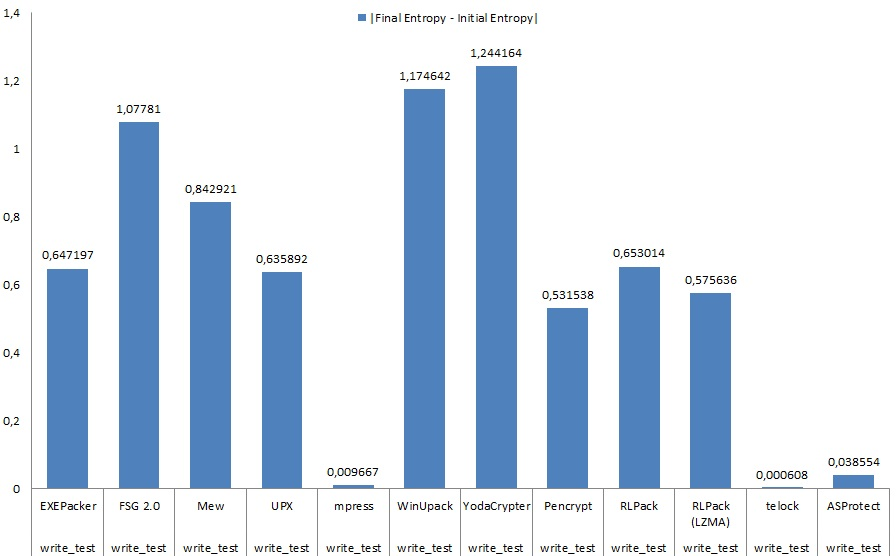
\includegraphics [width=\textwidth]{./pictures/Entropy Threshold Survey Results.jpg}
	\end{center}
	\caption{Entropy Threshold Survey Results}
	\label{Entropy Threshold Survey Results}
\end{figure}
A threshold of 0.6 is sufficient to cover almost all the packers
\item jump outer section heuristic: for each executed instruction we keep track of the \ac{EIP} of the previous one. In this way we can retrieve the section in which the previous instruction was located and compare it to the section of the current one. If these two are not equal we set the \textit{jump outer section} flag
\item long jump heuristic: as in the previous case we take advantage of tracking the previous instruction's \ac{EIP}. In this case we simply compute the difference between the previous and the current \ac{EIP}: 
\begin{equation}
difference = \left|current\_eip - previous\_eip\right|
\end{equation}
If this difference is above a given threshold we set the \textit{long jump} flag in the output report
 \item pushad popad heuristic: during the execution of the binary we have two flags indicating if we have encountered a \textit{pushad} or a \textit{popad}. For every instruction we check if it is one of the previous two and if so we set the corresponding flag. Then, when we produce a dump, if both flags are active, we set the \textit{pushad popad} flag in the output report
\item init function call heuristic: the aim of this heuristic is to search through the dumped code for calls to functions commonly used in the body of the malware and not in the unpacker stub. We achieve this result by using an IDAPython script: using IDA we are able to read the list of the imports of the dump and to confront it with a list of "suspicious" functions selected by us. Then we count the number of detected functions and write it in the output report
\end{itemize} 

\paragraph{}
At the end of the execution of our tool we have a report which contains a line for each dump that lists the results of every heuristic, as well as the dump number, a string that says if the \textit{Import Directory} is probably reconstructed or not, the \ac{OEP}, the begin and the end addresses of the \textit{Write Interval} considered for the dump. We use these information to choose the best dump as follow:
\begin{itemize}
\item first we check if the \textit{Import Directory} is probably reconstructed
\item is so, we count the number of the "suspicious" functions detected and the number of active heuristics' flags
\item if the previous numbers are the best result until this moment, we save this dump number, eventually rewriting another one saved before
\item at the end of the procedure we choose the saved dump number as the one that has the greatest chance to work
\end{itemize}
If no dump has its \textit{Import Directory} reconstructed, we return the value "-1".